%%%%%%%%%%%%%%%%%%%%%%%%%%%%%%%%%%%%%%%%%%%%%%%%%%%%%%%%%%%%%%%%%%%%%%%%%%
%
% Plantilla para libro de texto de matemáticas.
%
% Esta plantilla ha sido desarrollada desde cero, pero utiliza algunas partes
% del código de la plantilla original utilizada en apuntesDGIIM
% (https://github.com/libreim/apuntesDGIIM), basada a su vez en las plantillas
% 'Short Sectioned Assignment' de Frits Wenneker (http://www.howtotex.com),
% 'Plantilla de Trabajo' de Mario Román y 'Plantilla básica de Latex en Español'
% de Andrés Herrera Poyatos (https://github.com/andreshp). También recoge
% ideas de la plantilla 'Multi-Purpose Large Font Title Page' de
% Frits Wenneker y Vel (vel@latextemplates.com).
%
% Licencia:
% CC BY-NC-SA 4.0 (https://creativecommons.org/licenses/by-nc-sa/4.0/)
%
%%%%%%%%%%%%%%%%%%%%%%%%%%%%%%%%%%%%%%%%%%%%%%%%%%%%%%%%%%%%%%%%%%%%%%%%%

% ---------------------------------------------------------------------------
% CONFIGURACIÓN BÁSICA DEL DOCUMENTO
% ---------------------------------------------------------------------------

%\documentclass[11pt, a4paper, twoside]{article} % Usar para imprimir
\documentclass[10pt, a4paper]{article}

\usepackage[hyphens]{url}
\linespread{1.3}            % Espaciado entre líneas.
\setlength\parindent{0pt}   % No indentar el texto por defecto.
\setlength\parskip{7pt}

\usepackage{multirow}
\usepackage{xcolor,colortbl}
\usepackage{fancyvrb,newverbs,xcolor}
\usepackage{lipsum}% just for this example

\definecolor{cverbbg}{gray}{0.93}

\newenvironment{cverbatim}
 {\SaveVerbatim{cverb}}
 {\endSaveVerbatim
  \flushleft\fboxrule=0pt\fboxsep=.5em
  \colorbox{cverbbg}{\BUseVerbatim{cverb}}%
  \endflushleft
}
\newenvironment{lcverbatim}
 {\SaveVerbatim{cverb}}
 {\endSaveVerbatim
  \flushleft\fboxrule=0pt\fboxsep=.5em
  \colorbox{cverbbg}{%
    \makebox[\dimexpr\linewidth-2\fboxsep][l]{\BUseVerbatim{cverb}}%
  }
  \endflushleft
}

\newcommand{\ctexttt}[1]{\colorbox{cverbbg}{\texttt{#1}}}
\newverbcommand{\cverb}
  {\setbox\verbbox\hbox\bgroup}
  {\egroup\colorbox{cverbbg}{\box\verbbox}}

\usepackage[normalem]{ulem}
\usepackage{cancel}
\newcommand\dout{\bgroup \markoverwith{\rule[0.2ex]{0.1pt}{0.4pt}\rule[0.8ex]{0.1pt}{0.4pt}}\ULon}
\def\dout{\bgroup
 \markoverwith{\lower-0.35ex\hbox
 {\kern-.03em\vbox{\hrule width.2em\kern0.45ex\hrule}\kern-.03em}}%
 \ULon}
\MakeRobust\dout


% ---------------------------------------------------------------------------
% PAQUETES BÁSICOS
% ---------------------------------------------------------------------------

% IDIOMA
\usepackage[utf8]{inputenc}
\usepackage[spanish, es-tabla, es-lcroman, es-noquoting]{babel}

% MATEMÁTICAS
\usepackage{amsmath}    % Paquete básico de matemáticas
\usepackage{amsthm}     % Teoremas
\usepackage{mathrsfs}   % Fuente para ciertas letras utilizadas en matemáticas

% FUENTES
\usepackage{newpxtext, newpxmath}   % Fuente similar a Palatino
\usepackage{FiraSans}                 % Fuente sans serif
\usepackage[T1]{fontenc}
\usepackage[italic]{mathastext}     % Utiliza la fuente del documento
                                    % en los entornos matemáticos

% MÁRGENES
\usepackage[margin=2.5cm, top=3cm]{geometry}

% LISTAS
\usepackage{enumitem}       % Mejores listas
\setlist{leftmargin=.5in}   % Especifica la indentación para las listas.

% Listas ordenadas con números romanos (i), (ii), etc.
\newenvironment{nlist}
{\begin{enumerate}
    \renewcommand\labelenumi{(\emph{\roman{enumi})}}}
  {\end{enumerate}}

%  OTROS
\usepackage[hidelinks]{hyperref}   % Enlaces
\usepackage{graphicx}   % Permite incluir gráficos en el documento
\usepackage{relsize}

% LISTINGS
\usepackage{listings}
\usepackage{xcolor}     % Permite definir y utilizar colores
\usepackage{lipsum}
\usepackage{courier}

% Fijar tabla a posición
\usepackage{array}
\newcolumntype{L}[1]{>{\raggedright\let\newline\\\arraybackslash\hspace{0pt}}m{#1}}
\newcolumntype{C}[1]{>{\centering\let\newline\\\arraybackslash\hspace{0pt}}m{#1}}
\newcolumntype{R}[1]{>{\raggedleft\let\newline\\\arraybackslash\hspace{0pt}}m{#1}}


% Colores para los bloques de código
\definecolor{codegreen}{rgb}{0,0.6,0}
\definecolor{codegray}{rgb}{0.5,0.5,0.5}
\definecolor{codepurple}{rgb}{0.58,0,0.82}
\definecolor{backcolour}{rgb}{0.95,0.95,0.92}
\lstdefinestyle{mystyle}{
	backgroundcolor=\color{backcolour},   
	commentstyle=\color{codegreen},
	keywordstyle=\color{blue},
	numberstyle=\tiny\color{codegray},
	stringstyle=\color{codepurple},
	basicstyle=\footnotesize\ttfamily,
	breakatwhitespace=false,         
	breaklines=true,                 
	captionpos=b,                    
	keepspaces=true,                 
	numbers=left,                    
	numbersep=5pt,                  
	showspaces=false,                
	showstringspaces=false,
	showtabs=false,                  
	tabsize=4
}
\lstset{style=mystyle}

%\lstset{basicstyle=\footnotesize\ttfamily,breaklines=true}
%\lstset{framextopmargin=50pt,frame=bottomline}
 
% ---------------------------------------------------------------------------
% COMANDOS PERSONALIZADOS
% ---------------------------------------------------------------------------

% \equalto
\newcommand{\verteq}{\rotatebox{90}{$\,=$}}
\newcommand{\equalto}[2]{\underset{\scriptstyle\overset{\mkern4mu\verteq}{#2}}{#1}}


% ---------------------------------------------------------------------------
% COLORES
% ---------------------------------------------------------------------------

\definecolor{50}{HTML}{e8f5e9}
\definecolor{100}{HTML}{c8e6c9}
\definecolor{200}{HTML}{a5d6a7}
\definecolor{300}{HTML}{81c784}
\definecolor{400}{HTML}{66bb6a}
\definecolor{500}{HTML}{4caf50}
\definecolor{600}{HTML}{43a047}
\definecolor{700}{HTML}{388e3c}
\definecolor{800}{HTML}{2e7d32}
\definecolor{900}{HTML}{1b5e20}

% ---------------------------------------------------------------------------
% DISEÑO DE PÁGINA
% ---------------------------------------------------------------------------

\usepackage{pagecolor}
\usepackage{afterpage}

% ---------------------------------------------------------------------------
% CABECERA Y PIE DE PÁGINA
% ---------------------------------------------------------------------------

\usepackage{fancyhdr}   % Paquete para cabeceras y pies de página

% Indica que las páginas usarán la configuración de fancyhdr
\pagestyle{fancy}
\fancyhf{}

% Representa la sección de la cabecera
\renewcommand{\sectionmark}[1]{%
\markboth{#1}{}}

% Representa la subsección de la cabecera
\renewcommand{\sectionmark}[1]{%
\markright{#1}{}}

% Parte derecha de la cabecera
\fancyhead[LE,RO]{\sffamily\textsl{DGIIMCoin. Creando una criptomoneda} \hspace{1em}  \textcolor{500}{\rule[-0.4ex]{0.2ex}{1.2em}} \hspace{1em} \thepage}


\let\Oldpart\part
\newcommand{\parttitle}{}
\renewcommand{\part}[1]{\pagebreak\Oldpart{#1}\renewcommand{\parttitle}{#1}}

% Parte izquierda de la cabecera
\fancyhead[RE,LO]{\sffamily{\parttitle}}

% Elimina la línea de la cabecera
\renewcommand{\headrulewidth}{0pt}

% Controla la altura de la cabecera para que no haya errores
\setlength{\headheight}{14pt}

% ---------------------------------------------------------------------------
% TÍTULOS DE PARTES Y SECCIONES
% ---------------------------------------------------------------------------

\usepackage{titlesec}

% Estilo de los títulos de las partes
\titleformat{\part}[hang]{\Huge\bfseries\sffamily}{\thepart\hspace{20pt}\textcolor{500}{|}\hspace{20pt}}{0pt}{\Huge\bfseries}
\titlespacing*{\part}{0cm}{-2em}{2em}[0pt]

% Reiniciamos el contador de secciones entre partes (opcional)
\makeatletter
\@addtoreset{section}{part}
\makeatother

% Estilo de los títulos de las secciones, subsecciones y subsubsecciones
\titleformat{\section}
  {\Large\bfseries\sffamily}{\thesection}{1em}{}

\titleformat{\subsection}
  {\Large\sffamily}{\thesubsection}{1em}{}[\vspace{.5em}]

\titleformat{\subsubsection}
  {\sffamily}{\thesubsubsection}{1em}{}

% ---------------------------------------------------------------------------
% ENTORNOS PERSONALIZADOS
% ---------------------------------------------------------------------------

\usepackage{mdframed}

%% DEFINICIONES DE LOS ESTILOS

% Nuevo estilo para definiciones
\newtheoremstyle{definition-style}  % Nombre del estilo
{}                                  % Espacio por encima
{}                                  % Espacio por debajo
{}                                  % Fuente del cuerpo
{}                                  % Identación
{\bf\sffamily}                      % Fuente para la cabecera
{.}                                 % Puntuación tras la cabecera
{.5em}                              % Espacio tras la cabecera
{\thmname{#1}\thmnumber{ #2}\thmnote{ (#3)}}  % Especificación de la cabecera

% Nuevo estilo para notas
\newtheoremstyle{remark-style}
{10pt}
{10pt}
{}
{}
{\itshape \sffamily}
{.}
{.5em}
{}

% Nuevo estilo para teoremas y proposiciones
\newtheoremstyle{theorem-style}
{}
{}
{}
{}
{\bfseries \sffamily}
{.}
{.5em}
{\thmname{#1}\thmnumber{ #2}\thmnote{ (#3)}}

% Nuevo estilo para ejemplos
\newtheoremstyle{example-style}
{10pt}
{10pt}
{}
{}
{\bf \sffamily}
{}
{.5em}
{\thmname{#1}\thmnumber{ #2.}\thmnote{ #3.}}

% Nuevo estilo para la demostración

\makeatletter
\renewenvironment{proof}[1][\proofname] {\par\pushQED{\qed}\normalfont\topsep6\p@\@plus6\p@\relax\trivlist\item[\hskip\labelsep\itshape\sffamily#1\@addpunct{.}]\ignorespaces}{\popQED\endtrivlist\@endpefalse}
\makeatother

%% ASIGNACIÓN DE LOS ESTILOS

% Teoremas, proposiciones y corolarios
\newtheoremstyle{theorem-style}{}{}{}{}{}{}{ }{}
\theoremstyle{theorem-style}
\newtheorem*{datos}{}
\theoremstyle{theorem-style}
\newtheorem{nth}{Teorema}[section]
\newtheorem{nprop}{Proposición}[section]
\newtheorem{ncor}{Corolario}[section]
\newtheorem{lema}{Lema}[section]

% Definiciones
\theoremstyle{definition-style}
\newtheorem{ndef}{Definición}[section]

% Notas
\theoremstyle{remark-style}
\newtheorem*{nota}{Nota}

% Ejemplos
\theoremstyle{example-style}
\newtheorem{ejemplo}{Ejemplo}[section]

% Ejercicios y solución
\theoremstyle{definition-style}
\newtheorem{ejer}{Ejercicio}[section]

\theoremstyle{remark-style}
\newtheorem*{sol}{Solución}

%% MARCOS DE LOS ESTILOS

% Configuración general de mdframe, los estilos de los teoremas, etc
\mdfsetup{
  skipabove=1em,
  skipbelow=1em,
  innertopmargin=1em,
  innerbottommargin=1em,
  splittopskip=2\topsep,
}

% Definimos los marcos de los estilos


\mdfdefinestyle{datos-frame}{
	linewidth=2pt, %
	linecolor= 500, %
	topline=false, %
	bottomline=false, %
	rightline=false,%
	leftmargin=0em, %
	innerleftmargin=1em, %
	innerrightmargin=1em,
	rightmargin=0em, %
}%
\mdfdefinestyle{nth-frame}{
	linewidth=2pt, %
	linecolor= 500, %
	topline=false, %
	bottomline=false, %
	rightline=false,%
	leftmargin=0em, %
	innerleftmargin=1em, %
  innerrightmargin=1em,
	rightmargin=0em, %
}%

\mdfdefinestyle{nprop-frame}{
	linewidth=2pt, %
	linecolor= 300, %
	topline=false, %
	bottomline=false, %
	rightline=false,%
	leftmargin=0pt, %
	innerleftmargin=1em, %
	innerrightmargin=1em,
	rightmargin=0pt, %
}%

\mdfdefinestyle{ndef-frame}{
	linewidth=2pt, %
	linecolor= 500, %
	backgroundcolor= 50,
	topline=false, %
	bottomline=false, %
	rightline=false,%
	leftmargin=0pt, %
	innerleftmargin=1em, %
	innerrightmargin=1em,
	rightmargin=0pt, %
}%

\mdfdefinestyle{ejer-frame}{
	linewidth=2pt, %
	linecolor= 300, %
	backgroundcolor= 50,
	topline=false, %
	bottomline=false, %
	rightline=false,%
	leftmargin=0pt, %
	innerleftmargin=1em, %
	innerrightmargin=1em,
	rightmargin=0pt, %
}%

\mdfdefinestyle{ejemplo-frame}{
	linewidth=0pt, %
	linecolor= 300, %
	leftline=false, %
	rightline=false, %
	leftmargin=0pt, %
	innerleftmargin=1.3em, %
	innerrightmargin=1em,
	rightmargin=0pt, %
	innertopmargin=0em,%
	innerbottommargin=0em, %
	splittopskip=\topskip, %
}%

% Asignamos los marcos a los estilos
\surroundwithmdframed[style=nth-frame]{nth}
\surroundwithmdframed[style=datos-frame]{datos}
\surroundwithmdframed[style=nprop-frame]{nprop}
\surroundwithmdframed[style=nprop-frame]{ncor}
\surroundwithmdframed[style=ndef-frame]{ndef}
\surroundwithmdframed[style=ejer-frame]{ejer}
\surroundwithmdframed[style=ejemplo-frame]{ejemplo}
\surroundwithmdframed[style=ejemplo-frame]{sol}

% ---------------------------------------------------------------------------
% CONFIGURACIÓN DE LA PORTADA
% ---------------------------------------------------------------------------

\newcommand{\asignatura}{Fundamentos de Redes}

\newcommand{\autor}{Miguel Ángel Fernández Gutiérrez\\Pedro Gallego López}

\newcommand{\grado}{Doble Grado en Ingeniería Informática y Matemáticas}

\newcommand{\universidad}{Universidad de Granada}

% ---------------------------------------------------------------------------
% CONFIGURACIÓN PERSONALIZADA
% ---------------------------------------------------------------------------

%%%%%%%%%%%%%%%%%%%%%%%%%%%%%%%%%%%%%%%%%%%%%%%%%%%%%%%%%%%%%%%%%%%%%%%%%%%%%
% ---------------------------------------------------------------------------
% COMIENZO DEL DOCUMENTO
% ---------------------------------------------------------------------------
%%%%%%%%%%%%%%%%%%%%%%%%%%%%%%%%%%%%%%%%%%%%%%%%%%%%%%%%%%%%%%%%%%%%%%%%%%%%%

\begin{document}

% ---------------------------------------------------------------------------
% PORTADA EXTERIOR
% ---------------------------------------------------------------------------

\newpagecolor{500}\afterpage{\restorepagecolor} % Color de la página
\begin{titlepage}

  % Título del documento
	\parbox[t]{\textwidth}{
			\raggedright % Texto alineado a la izquierda
			\fontsize{40pt}{40pt}\selectfont\sffamily\color{white}{
				
\includegraphics[width=10cm]{./resources/logo_white.png}\\
				\textbf{\Huge{Creando una criptomoneda}}\\\huge{Fundamentos de Redes\\[-1cm]\Large{Seminarios}}
      }
	}

	\vfill

	%% Autor e información del documento
	\parbox[t]{\textwidth}{
		\raggedright % Texto alineado a la izquierda
		\sffamily\large\color{white}
		\grado\\
		{\Large \autor }\\[15pt]
		
\includegraphics[width=130pt]{ugrlogo.pdf}
	}

\end{titlepage}

% ---------------------------------------------------------------------------
% PÁGINA DE LICENCIA
% ---------------------------------------------------------------------------

\thispagestyle{empty}
\null
\vfill

%% Información sobre la licencia
\parbox[t]{\textwidth}{
  
\includegraphics{by-nc-sa.pdf}\\[4pt]
  \raggedright % Texto alineado a la izquierda
  \sffamily\large
  {\Large Este trabajo se distribuye bajo una licencia CC BY-NC-SA 4.0.}\\[4pt]
  Eres libre de distribuir y adaptar el material siempre que reconozcas a los\\
  autores originales del documento, no lo utilices para fines comerciales\\
  y lo distribuyas bajo la misma licencia.\\[4pt]
  \texttt{creativecommons.org/licenses/by-nc-sa/4.0/}
}

% ---------------------------------------------------------------------------
% PORTADA INTERIOR
% ---------------------------------------------------------------------------

\begin{titlepage}

  % Título del documento
  \parbox[t]{\textwidth}{
  	\raggedright % Texto alineado a la izquierda
  	\fontsize{40pt}{40pt}\selectfont\sffamily\color{500}{
				
\includegraphics[width=10cm]{./resources/logo_dark.png}\\
				\textbf{\Huge{Creando una criptomoneda}}\\\huge{Fundamentos de Redes\\[-1cm]\Large{Seminarios}}
  	}
  }

	\vfill
	
	%% Autor e información del documento
	\parbox[t]{\textwidth}{
		\raggedright % Texto alineado a la izquierda
		\sffamily\large
		\grado\\
		{\Large \autor }\\[15pt]
		
\includegraphics[width=130pt]{ugrlogo-dark.pdf}
	}

\end{titlepage}

% ---------------------------------------------------------------------------
% ÍNDICE
% ---------------------------------------------------------------------------

\thispagestyle{empty}
\tableofcontents
\newpage

% ---------------------------------------------------------------------------
% CONTENIDO
% ---------------------------------------------------------------------------

\part{¿Qué es una criptomoneda?}

Bitcoin es una de las \textbf{criptomonedas} más conocidas. Sepamos bien
cómo funciona o no, todos hemos oído hablar de Bitcoin. Sin embargo, hay
muchas otras, que se basan en los mismos principios básicos. Por tanto,
para explicar las criptomonedas, veamos cuáles son estos principios.

Supongamos que queremos crear una criptomoneda, \textbf{\emph{DGIIMCoin}}. La
primera pregunta sería para qué, y la segunda --en caso de que el para
qué nos haya convencido-- es qué necesitamos para ello.

\begin{center}
	
\includegraphics[width=10cm]{./resources/logo.png}
\end{center}

Crear todo esto tendría sentido si queremos crear un sistema anónimo,
descentralizado y seguro para intercambiar dinero o información. Veamos
bien qué quiere decir esto:

\begin{itemize}
\itemsep1pt\parskip0pt\parsep0pt
\item
  \textbf{Anónimo:} los usuarios deben ser identificables para el sistema, pero
  su identidad debe ser custodiada con recelo.
\item
  \textbf{Descentralizado:} los sistemas convencionales depositan la confianza de
  instituciones en terceros --i.e. Amazon en el envío de bienes, un banco, etc.--,
  en el caso de las criptomonedas su estado es mantenido gracias al consenso de
  los usuarios.
\item
  \textbf{Seguro:} el sistema no permite la realización de transacciones fraudulentas.
\end{itemize}

Bien, para todo esto nuestro sistema debería tener una serie de
requisitos:

\begin{enumerate}
\def\labelenumi{\arabic{enumi}.}
\itemsep1pt\parskip0pt\parsep0pt
\item[\emph{Req. 1.}]
  El sistema no requiere de una \textbf{autoridad central}: su estado es
  mantenido mediante un \textbf{consenso} distribuido.
\item[\emph{Req. 2.}]
  El sistema mantiene un \textbf{seguimiento} de todas las unidades de
  la criptomoneda y de sus propietarios.
\item[\emph{Req. 3.}]
  El sistema define si se pueden crear \textbf{nuevas unidades} de la
  criptomoneda. Si esto es así, el sistema debe definir las
  circunstancias de su origen y cómo determinar quién será el
  propietario de éstas.
\item[\emph{Req. 4.}]
  La propiedad de las monedas puede probarse de forma exclusivamente
  \textbf{criptográfica}.
\item[\emph{Req. 5.}]
  El sistema permite la realización de \textbf{transacciones} de forma
  controlada.
\end{enumerate}

Nuestro sistema, por tanto, girará en torno a las siguientes ideas clave:

\begin{enumerate}
\itemsep1pt\parskip0pt\parsep0pt
\item
  \textbf{Descentralización.}
\item
  \textbf{Firmas digitales.}
\item
  \textbf{La contabilidad (\emph{ledger}) es la propia moneda.}
\item
  \textbf{Mecanismo de consenso.}
\item
  \textbf{Blockchain.}
\end{enumerate}

Explicaremos cada una de ellas con más detalle.

\section{Descentralización: redes
P2P}\label{compartiendo-informaciuxf3n-de-forma-descentralizada-redes-p2p}

Para poder cumplir los dos primeros requisitos de nuestra lista,
eliminando así autoridades centralizadas, temos ya una solución
disponible: las \textbf{redes \emph{peer-to-peer}}, o \textbf{redes
P2P}.

La idea principal de estas redes es que la información se comparta de
igual a igual, al contrario a las redes cliente-servidor. En este caso,
todos los ordenadores tienen el mismo peso.

\subsection{Características de las redes P2P}

Una red \textbf{\emph{peer-to-peer}} (P2P) es una red de nodos en la que todos o algunos aspectos funcionan sin clientes ni servidores fijos, sino que cada nodo actúa simultáneamente como cliente y servidor respecto a los demás nodos de la red, todos ellos por igual. Las redes P2P permiten el intercambio directo de información, en cualquier formato, entre los ordenadores interconectados.

Las redes \emph{peer-to-peer} aprovechan, administran y optimizan el uso del ancho de banda de los demás usuarios de la red por medio de la conectividad entre los mismos, y obtienen así más rendimiento en las conexiones y transferencias que con algunos métodos centralizados convencionales, donde una cantidad relativamente pequeña de servidores provee el total del ancho de banda y recursos compartidos para un servicio o aplicación.

Los rasgos a destacar de este tipo de red son:

\begin{itemize}
\def\labelenumi{\arabic{enumi}.}
\itemsep1pt\parskip0pt\parsep0pt
\item
  \textbf{Escalabilidad.} Las redes P2P tienen un alcance mundial con cientos de
millones de usuarios potenciales. En general, lo deseable es que cuantos
más nodos estén conectados a una red P2P, mejor será su funcionamiento.
Así, cuando los nodos llegan y comparten sus propios recursos, los recursos totales del sistema aumentan. Esto es radicalmente opuesto al caso de la arquitectura servidor-cliente con un sistema fijo de servidores, en los cuales la adición de clientes podría significar una transferencia de datos más lenta para todos los usuarios.
\item
  \textbf{Descentralización.} Estas redes por definición son descentralizadas y
todos los nodos son iguales. No existen nodos con funciones especiales, y
por tanto ningún nodo es imprescindible para el funcionamiento de la red.
Nótese sin embargo que, en realidad, algunas redes comúnmente llamadas P2P no cumplen esta
característica, como en Napster, eDonkey, BitTorrent, etc.
\item
  \textbf{Distribución de costes entre los usuarios.} Se comparten o donan
recursos a cambio de recursos. Según la aplicación de la red, los recursos
pueden ser archivos, ancho de banda, ciclos de proceso o almacenamiento
de disco.
\item
	\textbf{Robustez.} La naturaleza distribuida de las redes \emph{peer-to-peer} también
incrementa la robustez en caso de haber fallos en la réplica excesiva de
los datos hacia múltiples destinos, y en sistemas P2P puros permitiendo a
los peers encontrar la información sin hacer peticiones a ningún servidor
centralizado de indexado. En el último caso, no hay ningún punto
singular de falla en el sistema.
\item
	\textbf{Anonimato.} Es deseable que en estas redes quede anónimo el autor de un
contenido, el editor, el lector, el servidor que lo alberga y la petición para
encontrarlo, siempre que así lo necesiten los usuarios. Muchas veces el
derecho al anonimato y los derechos de autor son incompatibles entre sí,
y la industria propone mecanismos como el DRM para limitar ambos.
\item
	\textbf{Seguridad.} Es una de las características deseables de las redes P2P
menos implementada. Los objetivos de un P2P seguro serían identificar y
evitar los nodos maliciosos, evitar el contenido infectado, evitar el
espionaje de las comunicaciones entre nodos, creación de grupos seguros
de nodos dentro de la red y protección de los recursos de la red, entre otros. La
mayor parte de estas características aún están bajo investigación, pero los
mecanismos más prometedores son: cifrado multiclave, cajas de arena,
gestión de derechos de autor, etc.
\end{itemize}

\subsection{Topologías de las redes P2P}

Una red \emph{peer-to-peer} puede tener diversas topologías diferentes:

\begin{itemize}
\def\labelenumi{\arabic{enumi}.}
\itemsep1pt\parskip0pt\parsep0pt
\item
  \textbf{Centralizada.} Se mantiene un directorio en un servidor central, al cual
las computadoras conectadas hacen peticiones para encontrar los nodos
que contienen los contenidos deseados. Su principal defecto es que ese
servidor central es un punto crítico.
\item
  \textbf{Descentralizada y estructurada}, también conocida como \textbf{P2P híbrida}. No existe un directorio en un servidor central, sino en varias
computadoras colocadas en lugares de la red que hacen fácil su acceso a
otras computadoras.
\item
	\textbf{Descentralizada y no estructurada.} No existen computadoras o nodos
que funcionen como controladores centrales de peticiones. Todos los
nodos funcionan como clientes y como servidores.
\end{itemize}

\begin{table}[h]
\begin{tabular}{ccc}
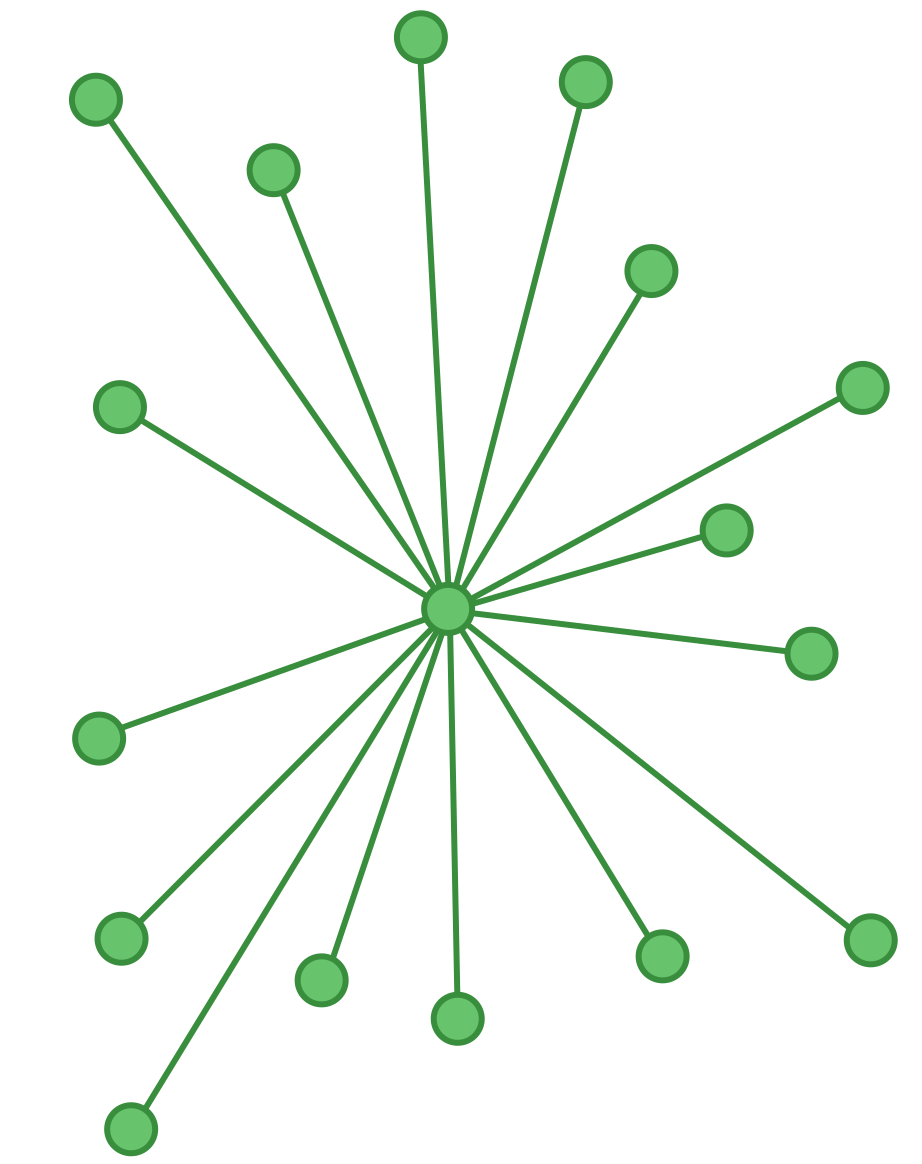
\includegraphics[width=5cm]{./resources/p2p1.png} & 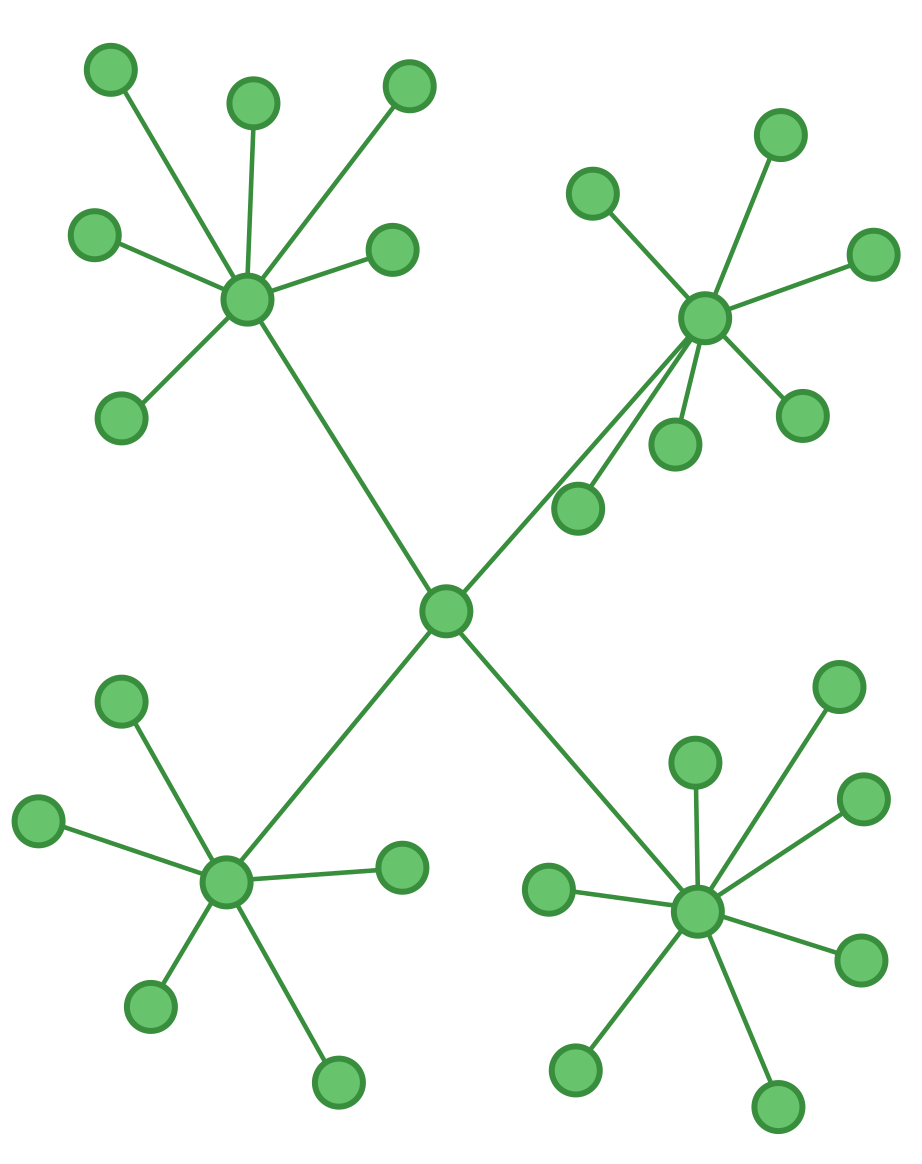
\includegraphics[width=5cm]{./resources/p2p2.png} & 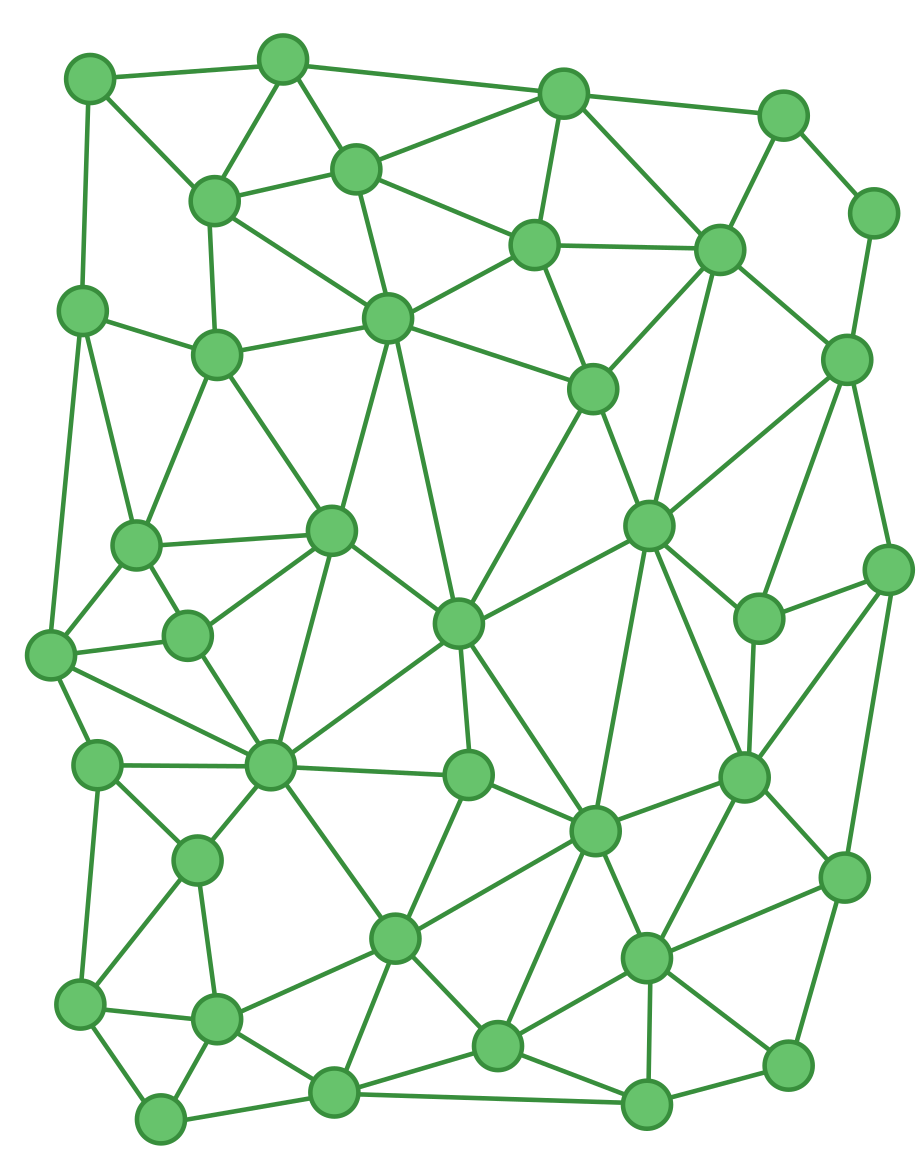
\includegraphics[width=5cm]{./resources/p2p3.png} \\
centralizada & descentralizada y estructurada & descentralizada y no estructurada
\end{tabular}
\end{table}

\subsection{Ventajas e inconvenientes de las redes P2P}

La principal ventaja que presenta P2P es la creación de grandes bases de datos de manera gratuita, ya que todos los ordenadores conectados en línea pueden descargarse archivos de otros ordenadores también conectados. Con el aumento de la velocidad de conexión de Internet, propiciada por la instalación del ADSL, los programas de intercambio de archivos y la frecuencia de este tipo de operaciones aumenta de forma considerable. 

Muchos de los programas P2P son gratuitos, lo cual los hace una opción atractiva para quienes buscan contenido gratuito (la legalidad de esa práctia es cuestionable). Existen programas P2P con contenido legal y que conllevan una suscripción  de pago, lo cual sigue siendo una buena opción si se busca un precio económico. Es por tanto la legalidad de las funcionalidades que te ofrece una red P2P determinada lo que puede cuestionar el uso de ésta.

En conclusión, tendríamos las siguientes ventajas:
\begin{itemize}
\def\labelenumi{\arabic{enumi}.}
\itemsep1pt\parskip0pt\parsep0pt
\item
  \textbf{Costo:} muchos de los programas P2P son gratuitos.
\item
  \textbf{Eficiencia:} compartir archivos en P2P es fácil y rápido.
\end{itemize}

Sin olvidar los inconvenientes:
\begin{itemize}
\def\labelenumi{\arabic{enumi}.}
\itemsep1pt\parskip0pt\parsep0pt
\item
  \textbf{Legalidad:} compartir archivos ilegales por estas redes.
\end{itemize}

En definitiva, podemos usar los protocolos P2P existentes para
implementar \emph{DGIIMCoin}. Genial, continuemos.
\section{Firmas digitales, criptografía y
\emph{hashing}}\label{firmas-digitales-criptografuxeda-y-hashing}

Para que nuestro sistema funcione son esenciales las \textbf{identidades
digitales}, es decir, formas de verificar que una transacción se ha
hecho realmente (alguien de verdad ha enviado dinero a otra persona).
Para eso, usamos la \textbf{criptografía}.

\subsection{Funciones hash}

En concreto, necesitaremos un algoritmo de \textbf{hashing}. Esencialmente, una función hash es una función que, dada una entrada de un tamaño arbitrario, da una salida de tamaño fijo, e ilegible.

\begin{center}
	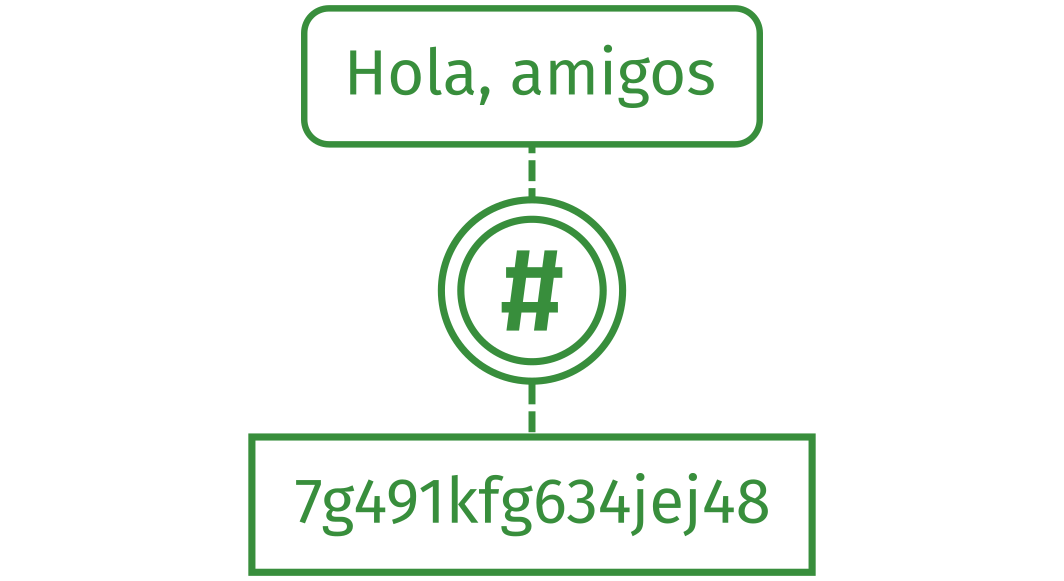
\includegraphics[width=10cm]{./resources/hash.png}
\end{center}

Una buena función hash debe garantizar:

\begin{enumerate}
\item
	La salida de la función hash debe tener un tamaño fijo (por ejemplo, en el caso de SHA256 el tamaño es de 256 bits).
\item
	Un mínimo cambio en la entrada debe producir un enorme cambio en la salida.
\item
	Una misma entrada siempre producirá la misma salida.
\item
	No debe haber forma alguna de revertir el cambio, es decir, de que a partir de la salida se pueda encontrar la entrada.
\item
	Calcular el valor hash debe ser rápido; no debe requerir de un gran trabajo computacional.
\end{enumerate}

Es importante mencionar que, aunque el número de valores hash posibles es limitado, las colisiones son muy poco probables, e incluso en caso de que se produzca alguna, sería imposible encontrar el patrón que dichas colisiones siguen.
\subsection{Firmas digitales}

Ahora bien, estas funciones son importantes especialmente a la hora de garantizar que las transacciones en el sistema son ciertas. Las funciones hash son utilizadas por algoritmos criptográficos que garantizan la veracidad de las transacciones.

Para asegurarnos de que nadie puede hacer una transacción en tu nombre, usaremos el concepto de \textbf{firma digital}. La mejor forma de hacerlo es mediante el método de \textbf{clave privada-clave pública}, también llamado \textbf{criptografía asimétrica}.

\begin{center}
	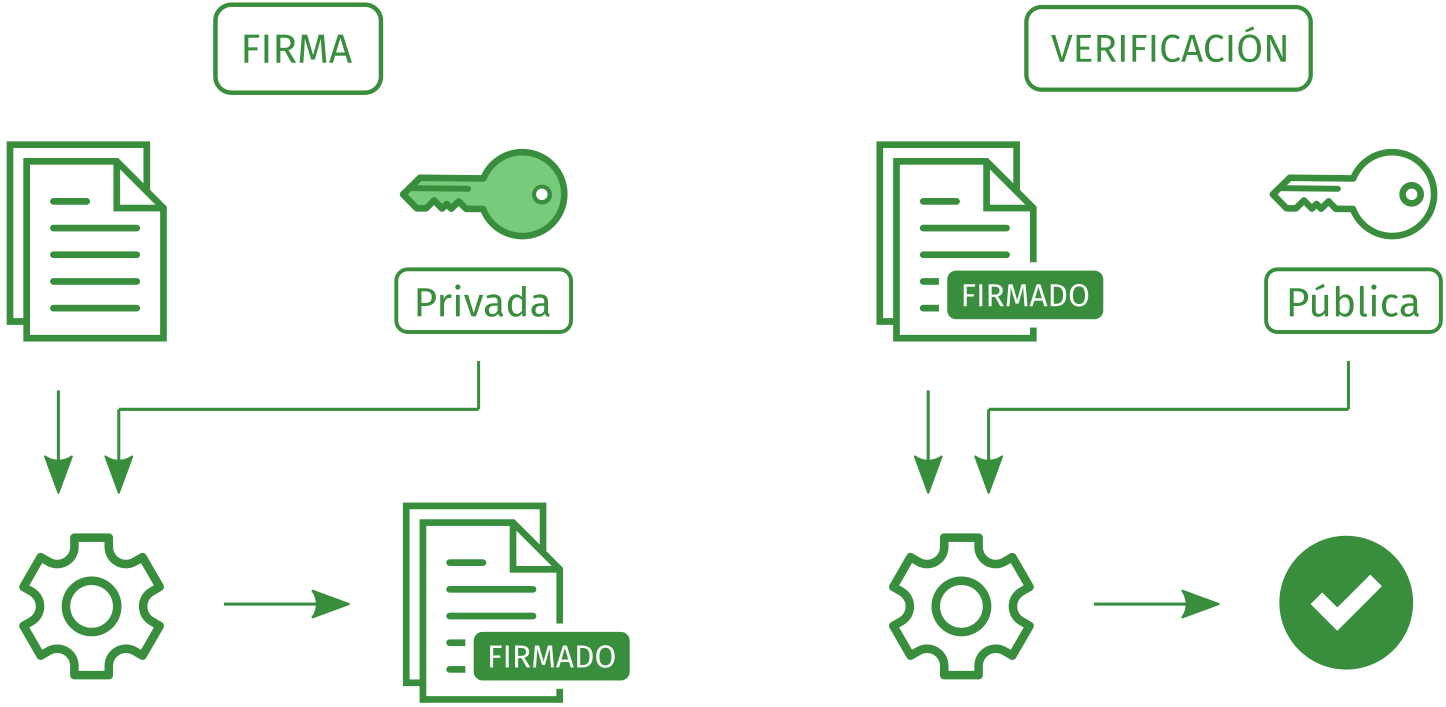
\includegraphics[width=13cm]{./resources/signing.png}
\end{center}

Cada usuario tendrá dicho conjunto de claves, cada una de ellas será un conjunto de bits determinado. Nos aseguraremos que nadie tiene acceso a nuestra clave privada. Para producir una firma, usaremos la siguiente función:
$$
Firmar(\textbf{Mensaje}, \textbf{Clave Privada}) = \textbf{Firma}
$$

Que dependa de la clave privada significa que tú eres el único capaz de firmar, y que también dependa del mensaje asegura que los mensajes no puedan modificarse una vez firmados, porque el resultado de esta función sería radicalmente diferente. Para comprobar nos basta usar la clave pública, pues ésta tiene una relación con la clave privada.
$$
Verificar(\textbf{Mensaje}, \textbf{Firma}, \textbf{Clave Pública}) = \begin{cases} true \\ false \end{cases}
$$

\section{Enviando transacciones a la
red}\label{enviando-transacciones-a-la-red}

Ya casi estamos. Hemos implementado comunicación P2P, mecanismos para
crear identidades digitales y formas para que los usuarios puedan firmar
y garantizar que la información es correcta. Ahora sólo nos queda enviar
información al sistema.

Como ya sabemos, no tenemos una autoridad central que valide cuánto
dinero tenemos, pero tampoco hace falta: aquí reside una de las ideas,
que la \textbf{contabilidad es la propia moneda}. Esto se debe a que
para saber cuánto dinero tenemos, simplemente nos basta con tener una
lista de todas las transacciones que hemos efectuado. Supongamos que tu
historial de transacciones contiene la información:

\begin{datos}
{\sffamily \textbf{Ejemplo.} Listado de transacciones de un usuario en \emph{DGIIMCoin}}\\
\begin{enumerate}
\def\labelenumi{\arabic{enumi}.}
\itemsep1pt\parskip0pt\parsep0pt
\vspace{-1.2cm}
\item[]
	\hspace{1cm}
\item
  Tengo 500\dout{D}.
\item
  Envío 20\dout{D} a alguien para unos apuntes de Modelos de
  Computación (incluiremos su clave pública).
\item
  Quiero enviar 1\dout{D} como impuesto de transacción al sistema (lo
  veremos más adelante).
\end{enumerate}
\end{datos}

Lo único que queda es usar la red P2P para enviar estas transacciones al
resto de usuarios del sistema, sin olvidar de firmarlas usando nuestra
clave privada. Tras esto, todo el mundo podrá ver la transacción (aunque las identidades de ambos estarán encriptadas).

Listo. Sin embargo, no tendrás los apuntes hasta que la red coincida en
que inicialmente tenías 500\dout{D}, y por tanto dicha transacción
puede efectuarse. Una vez que la transacción se valide, tu compañero te
dará los apuntes.

\section{El blockchain}\label{el-blockchain}

Para poder mantener nuestro sistema necesitamos tener un historial de las transacciones que han sido realizadas. Para esto, usamos la tecnología \textbf{blockchain}, que es esencialmente un conjunto de bloques que contienen información (que veremos más adelante), que son enlazados usando criptografía: cada bloque tiene un hash del bloque anterior, así como metadatos de su creación.

\begin{center}
	
\includegraphics[width=13cm]{./resources/blockchainoverview.png}
\end{center}

Esto precisamente hace que nuestro libro de cuentas público (\emph{public ledger}) sea resistente a modificaciones: la alteración de un bloque invalida todos los sucesivos. Aunque es posible efectuar estas alteraciones, esta tecnología es segura y tolerante a faltas bizantinas\footnote{La \textbf{tolerancia a faltas bizantinas} es la resistencia de un sistema informático a fallas de componentes electrónicos donde hay información imperfecta sobre si un componente falla. Es de especial importancia en sistemas distribuidos, como el que nos concierne.}.

\subsection{Los bloques}

Los bloques contienen un conjunto de transacciones que son hasheadas y codificadas en un \textbf{árbol de Merkle} (la estructura de datos que mantiene los enlaces entre los bloques mediante funciones hash).
\vspace{3cm}
\pagebreak

A veces dos bloques pueden ser creados de forma concurrente, generando un \emph{fork} temporal. Por esto, necesitaremos una forma de ``puntuar'' diferentes versiones, para que uno con una puntuación más alta pueda ser seleccionado antes que el resto. Los bloques no seleccionados para la inclusión son los denominados \textbf{bloques huérfanos}.

\begin{center}
	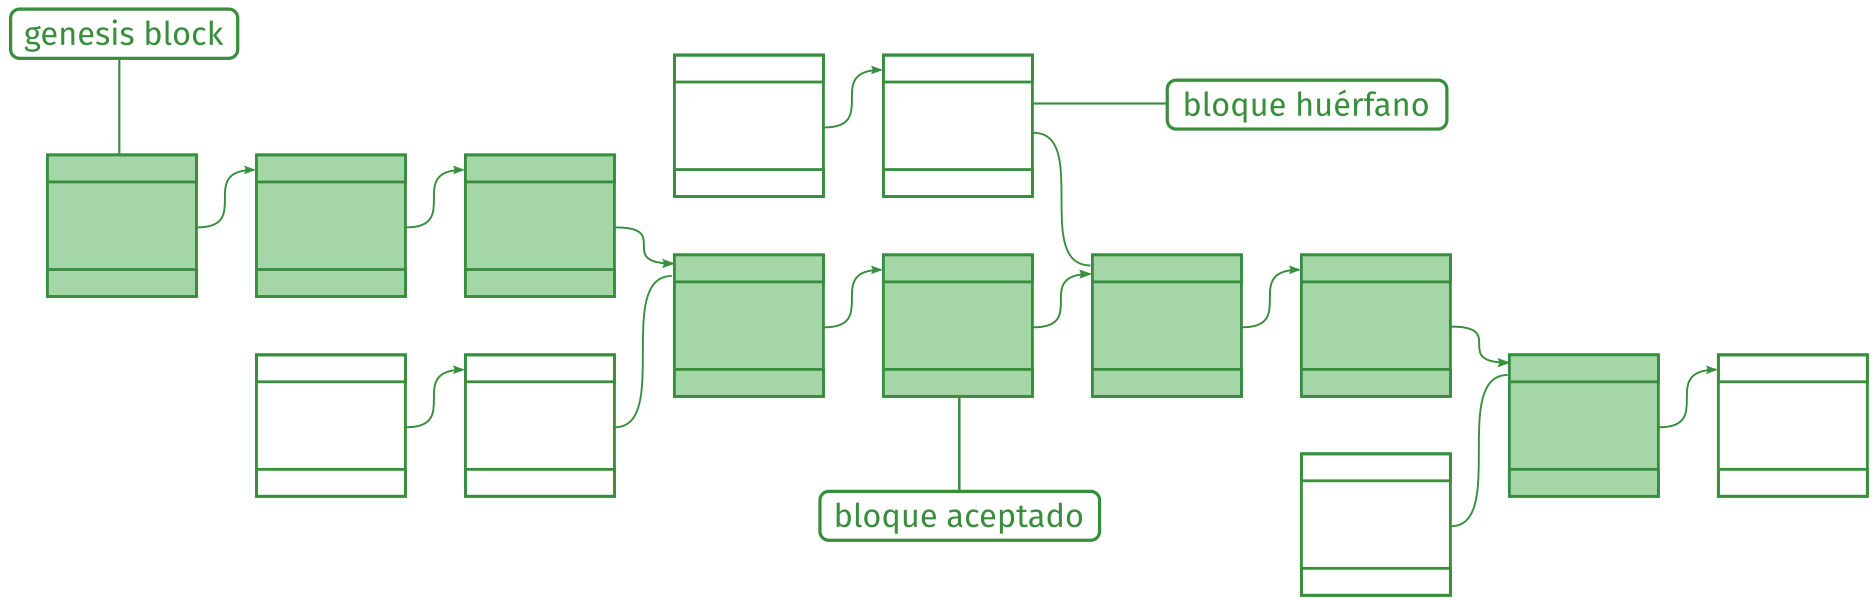
\includegraphics[width=16cm]{./resources/chain.png}
\end{center}

Más adelante, veremos la estructura exacta de estos bloques, en el caso de Bitcoin.


\section{Mecanismos de verificación de
transacciones: \emph{mining}}\label{mecanismos-de-verificaciuxf3n-de-transacciones}

Bien, ya que tenemos mecanismos para generar y guardar transacciones de forma descentralizada, nos falta el factor de la \textbf{confianza}: ¿cómo sabemos que una transacción es cierta?

Supongamos la siguiente situación: María debe pagarle 100\dout{D} a Jorge, y de hecho tiene el dinero disponible, pero quiere timar a Jorge haciéndole creer que en efecto se los ha pagado, enviando esta transacción a Jorge, pero no al resto de usuarios de nuestro sistema. Para Jorge, María habrá saldado sus deudas con él, mientras que realmente Jorge nunca tendrá ese dinero.

Para evitar esto, es necesario establecer un sistema mediante el cual se pueda establecer un criterio para discernir qué bloque de nuestro blockchain es más correcto. Deberíamos, por tanto, implementar en este momento un mecaniso de autenticación sustentado por el interés colectivo.\\

En nuestro blockchain hay unos actores especialmente destacables, que aportan una funcionalidad esencial para el buen funcionamiento de nuestra criptomoneda. Estos son los \textbf{mineros}, que son los encargados de crear bloques nuevos donde poder guardar las transacciones. Estos mineros no son otra cosa que un usuario de nuestra criptomoneda cuya aportación es potencia de cómputo a un problema matemático.

Pero, un segundo, \emph{¿un problema matemático en un bloque?} Efectivamente, como antes hemos comentado, tenemos una función hash SHA-256 (en el caso de Bitcoin), que tiene como output un número de 256 bits, es decir, se pueden generar $2^{256}$ resultados. Y es aquí donde se nos plantea el problema matemático:

\begin{datos}
\hspace{-0.115cm}Encontrar un número que, al ser introducido en la función hash junto con los datos del bloque que se quiere crear, el resultado sea un número que empiece por muchos 0.
\end{datos}

Nuestros mineros tratarán de resolver este problema y el número del minero que consiga más ceros será el escogido. Pero, ¿qué motivación tienen estos mineros para trabajar en formar bloques y no en corromperlos?

Pensemos en una forma de beneficiar a los que se ofrecen a hacer crecer a la comunidad. Obtendremos diversos esquemas para ello, y de ese modo hacer que la blockchain funcione de manera independiente, segura, transparente y democrática. Además, premia a los mineros con las mismas criptomonedas y promueve que sigan minando criptomonedas y que lo hagan de forma honesta.

\subsection{Proof-of-work (PoW)}

El esquema de \textbf{proof-of-work (PoW)}, o \textbf{prueba de trabajo}, es un algoritmo que premia a los participantes que resuelvan acertijos criptográficos para validar las transacciones y crear nuevos bloques. Este es el esquema que utiliza Bitcoin. \textbf{Tienen más posibilidad de resolver los acertijos aquellos mineros que tengan mayor poder computacional trabajando a disposición del sistema}. De esto el nombre del sistema, pues da prioridad a aquellos que más trabajan.

En este esquema, los mineros compiten por resolver los acertijos para crear nuevos bloques de la blockchain, en el caso de Bitcoin cada 10 minutos. Los mineros que inviertan más trabajo en crear los bloques tienen más posibilidades de encontrar la respuesta y como recompensa obtendrán criptomonedas.

Una de las mayores desventajas del PoW es que gasta mucha energía, pues se desperdicia el trabajo de todos los mineros que intentaron encontrar la respuesta correcta pero que no lo lograron.

\subsection{Proof-of-burn (PoB)}\label{proof-of-burn}

\textbf{Proof-of-burn (PoB)} es un algoritmo similar al de prueba de trabajo, pero con tasas reducidas de consumo de energía. El proceso de validación de bloques de las redes basadas en PoB no requiere el uso de recursos computacionales potentes y no depende de hardware minero potente (como los ASIC). En cambio, las criptomonedas se queman intencionadamente como una forma de ``invertir'' los recursos en la blockchain, por lo que los candidatos mineros no están obligados a invertir recursos físicos. En los sistemas PoB, \textbf{los mineros invierten en plataformas de minería virtual} (o potencia de minería virtual).

En otras palabras, al realizar quemas de monedas, los usuarios pueden demostrar su compromiso con la red, obtener el derecho a ``minar'' y validar las transacciones. Dado que el proceso de quemar monedas representa el poder de minería virtual, cuantas más monedas quema un usuario en favor del sistema, más poder de minería tiene, y por lo tanto mayores son las posibilidades de ser elegido como el siguiente validador de bloques.

En definitiva, el proceso de quemar monedas consiste en enviarlas a un público verificable donde se vuelven inaccesibles e inútiles. Normalmente, estas direcciones (también conocidas como \emph{eater addresses}\footnote{Más información en \url{https://www.blockchain.com/btc/address/1BitcoinEaterAddressDontSendf59kuE}}) se generan de forma aleatoria sin tener ninguna clave privada asociada a ellas. Naturalmente, el proceso de quema de monedas reduce la disponibilidad del mercado y crea una escasez económica, causando un aumento potencial en su valor. Pero más que eso, la quema de monedas es otra forma de invertir en la seguridad de la red.

\subsection{Proof-of-stake (PoS)}\label{proof-of-stake}

\textbf{Proof-of-stake (PoS)}, o \textbf{prueba de participación}, es un tipo de algoritmo de consenso que depende de la participación económica de un validador en la red. \textbf{La importancia de este sistema se centra en la propiedad de la moneda en cuestión}. No requiere trabajo o poder computacional, más bien requiere poseer la criptomoneda.


Tener criptomonedas en la cartera digital es aquello que refleja la participación de los usuarios y \textbf{tienen más poder en la criptomoneda los usuarios que tengan en su cuenta más criptomonedas durante más tiempo}.

Mientras más criptomonedas posean los usuarios, más poder de minería poseen para validar los bloques de blockchain y por lo tanto más criptomonedas recibirán como recompensa. Es un sistema que no desperdicia tanta energía como PoW.

Sin embargo, si un usuario compromete sus criptomonedas como prueba de participación, entonces no las puede gastar en otras cosas, por lo tanto, un inconveniente de este sistema es que podría inhibir la comercialización con las criptomonedas minadas.

\subsection{Proof-of-elapsed time (PoET)}\label{proof-of-elapsed-time}

En el caso del \textbf{proof-of-elapsed time (PoET)}, el algoritmo se basa en el principio de un sistema de lotería justo, donde cada nodo tiene la misma probabilidad de ganar. El mecanismo PoET se basa en distribuir las posibilidades de ganar de manera justa entre el mayor número de participantes de la red.

El funcionamiento del algoritmo PoET es el siguiente:

\begin{datos}
{\sffamily \textbf{Algoritmo.} Algoritmo PoET}\\
\begin{enumerate}
\def\labelenumi{\arabic{enumi}.}
\itemsep1pt\parskip0pt\parsep0pt
\vspace{-1.2cm}
\item[]
	\hspace{1cm}
\item
  Se requiere que cada nodo participante en la red espere un período de tiempo elegido al azar, y el primero en completar el tiempo de espera designado gana el nuevo bloque.
\item
  Cada nodo en la red blockchain genera un tiempo de espera aleatorio y se va a dormir durante esa duración especificada.
\item
	El nodo que tiene el menor tiempo de espera, se despierta y envía un nuevo bloque a la cadena de bloques, transmitiendo la información necesaria a toda la red de pares.
\item
  El mismo proceso se repite para el descubrimiento del siguiente bloque.
\end{enumerate}
\end{datos}

\subsection{Proof-of-importance (PoI)}\label{proof-of-importance}

\textbf{Proof-of-importance (PoI)}, o \textbf{prueba de importancia}, da prioridad a los mineros que tengan \textbf{mejor reputación en el sistema}. La reputación se mide por la cantidad de dinero invertido, el número de transacciones realizadas y la cantidad transferida en dichas transacciones. También se toma en cuenta para medirla la reputación de las cuentas con las que se realizan los intercambios. Este es el sistema que se utiliza para la criptomoneda NEM.\\

Por lo tanto, si María quisiera crear un bloque fraudulento para timar a Jorge, tendría que seguir con su mentira indefinidamente, algo que es casi imposible, ya que para ello debería equiparar su capacidad de cómputo a la del resto de mineros.

\section{Controlando la fuente de
dinero}\label{controlando-la-fuente-de-dinero}

Ahora bien, ¿de dónde viene el dinero en este tipo de sistemas? Tras la mayoría de las criptomonedas, la idea es que se genera más dinero conforme hay más trabajo, es decir, conforme hay más paquetes y más mineros. Este dinero se genera como recompensa al trabajo de los mineros, como hemos explicado antes.

Un caso particular es el de Bitcoin, en el que hay un límite superior de 21 millones de bitcoins. Todavía no se ha llegado a ese número, y se calcula que, al ritmo actual, llegaremos a él en el año 2140.

Este límite no se superará, sin embargo, debido a que la recompensa de los mineros va disminuyendo conforme hay más dinero en el sistema, llegando a ser una recompensa ausente.

Esta recompensa se calcula a partir de tres factores:
\begin{itemize}
\def\labelenumi{\arabic{enumi}.}
\itemsep1pt\parskip0pt\parsep0pt
\item
  \textbf{El dinero que ya hay en el sistema:} conforme nos acercamos a los 21 millones de bitcoins, la recompensa cada vez será menor.
\item
  \textbf{El trabajo computacional de los mineros:} conforme más mineros trabajan, más complicado es llegar a la solución (véase el factor siguiente). Esto también se tiene en cuenta a la hora de calcular la recompensa.
\item
  \textbf{La dificultad del mineo:} Bitcoin acepta bloques cada 10 minutos, y ajusta la dificultad (el número de ceros base) en función del número de mineros que haya, y del dinero que hay en la plataforma.
\end{itemize}

Una vez que lleguemos al límite, la importancia recaerá en las \textbf{tarifas de transacción}. Cada vez que un usuario realiza una transacción en Bitcoin, puede incluir una tarifa de transacción, que el minero obtendrá como recompensa, incentivando de esta forma el mineo. Además, debido a que el número de transacciones en un bloque de Bitcoin es limitado (realmente no se mide el número de transacciones, sino el ``peso'' de cada transacción)\footnote{Más información aquí: \url{https://bitcoinmagazine.com/guides/what-is-the-bitcoin-block-size-limit}}, los mineros insertarán en los bloques las transacciones más beneficiosas para ellos.


\hspace*{1cm}
\vspace{7cm}


\pagebreak
\part{Demo: Bitcoin Core}\label{demo-wireshark}

Para ejemplificar cuál es la estructura de los bloques de la blockchain de una criptomoneda, así como el protocolo de comunicación de red que se utiliza, usaremos la aplicación \textbf{Bitcoin Core}, la implementación oficial de Bitcoin, que puede ser usada como cartera.

\section{Procedimiento seguido}

Sencillamente, descargaremos \textbf{Bitcoin Core} de la página web oficial de Bitcoin: \url{https://bitcoin.org/en/bitcoin-core/}, y seguiremos las instrucciones que aparecen en el archivo descargado para ejecutar el cliente \texttt{bitcoin-qt}. Como es la primera vez que ejecutamos \texttt{bitcoin-qt}, se conectará con la red Bitcoin y se descargará todos los bloques de la blockchain: ¡más de 200GB! Pero no te preocupes, pararemos la descarga para poder inspeccionar algunos bloques. Además, durante esta descarga ejecutaremos \textbf{Wireshark} para escuchar los mensajes intercambiados en Bitcoin.

Los datos descargados, por defecto, serán guardados en

\hspace{1cm}\texttt{\textasciitilde/.bitcoin}

Analizaremos por tanto el resultado de lo descrito anteriormente desde dos perspectivas:

\begin{itemize}
\def\labelenumi{\arabic{enumi}.}
\itemsep1pt\parskip0pt\parsep0pt
\item
  \textbf{Los bloques:} analizaremos los bloques descargados por \texttt{bitcoin-qt} y veremos cómo los componentes de una criptomoneda explicados anteriormente están en éstos.
\item
  \textbf{Los mensajes:} veremos cómo funciona el protocolo de Bitcoin analizando los mensajes enviados y recibidos en Wireshark.
\end{itemize}

\section{Análisis de bloques}

Entraremos en el directorio \texttt{.bitcoin}. Vemos que tiene un subdirectorio llamado \texttt{blocks}.

\begin{table}[h]
\begin{tabular}{L{15.6cm}}
\cellcolor[gray]{0.9}
\begin{minipage}{3in}
\vspace{0.3cm}
\begin{Verbatim}[commandchars=\\\{\}]
$> pwd
~/.bitcoin
$> ls
banlist.dat  chainstate/  fee_estimates.dat  peers.dat
blocks/      debug.log    mempool.dat        wallets/
$> cd blocks; ls
blk00000.dat  blk00003.dat  index/        rev00002.dat  rev00005.dat
blk00001.dat  blk00004.dat  rev00000.dat  rev00003.dat
blk00002.dat  blk00005.dat  rev00001.dat  rev00004.dat
\end{Verbatim}
\vspace{0cm}
\end{minipage}
\end{tabular}
\end{table}

Cada archivo \cverb|blk00*.dat| es una colección de bloques de cierto tamaño. Analizaremos uno de ellos, por ejemplo, \cverb|blk00003.dat|.

Cada bloque sigue un formato especificado por Bitcoin:

\begin{table}[h]
\begin{tabular}{|C{4.5cm}|L{8.5cm}|C{1.7cm}|}
\hline
\multicolumn{1}{|c}{\cellcolor[HTML]{81c784}\textbf{Campo}} & \multicolumn{1}{|c}{\cellcolor[HTML]{81c784}\textbf{Descripción}} & \multicolumn{1}{|c|}{\cellcolor[HTML]{81c784}\textbf{Tamaño}}\\
\hline
Número mágico & El valor siempre es \texttt{0xD9B4BEF9} & 4 bytes \\
\hline
Tamaño de bloque & Longitud del bloque en bytes & 4 bytes \\
\hline
Cabecera de bloque & 6 elementos & 80 bytes \\
\hline
Contador de transacciones & Entero positivo (\texttt{var\_int}) & 1-9 bytes \\
\hline
Transacciones & La lista de transacciones (no vacía) & Variable \\
\hline
\end{tabular}
\end{table}

Veamos con más detalle cada uno de ellos.

\subsection{Número mágico}

El primer elemento es una secuencia de 4 bytes fija, el \textbf{número mágico}, cuyo valor siempre es \texttt{0xD9B4BEF9}. Como el protocolo de Bitcoin usa \emph{little endian}, la lectura del archivo binario resultará en la secuencia de bytes \texttt{0xF9 0xBE 0xB4 0xD9}. Haciendo \texttt{hexdump}:

\begin{table}[h]
\begin{tabular}{L{15.6cm}}
\cellcolor[gray]{0.9}
\begin{minipage}{3in}
\vspace{0.3cm}
\begin{Verbatim}[commandchars=\\\{\}]
$> hexdump -C -n 32 blk00003.dat
00000000  \textcolor{red}{f9 be b4 d9} c2 bf 00 00  01 00 00 00 47 0c 5f a9
00000010  f8 d7 29 d0 ec c7 04 d0  b7 d1 23 31 c5 f4 15 bd
00000020
\end{Verbatim}
\vspace{0cm}
\end{minipage}
\end{tabular}
\end{table}

\subsection{Tamaño de bloque}

El bloque es seguido por cuatro bytes, que especifican el tamaño del bloque en bytes. En nuestro caso, convertir de \emph{little endian} \texttt{0xC2BF0000} nos da \texttt{0x0000BFC2}, que convertido a decimal son 49090 bytes.

\begin{table}[h]
\begin{tabular}{L{15.6cm}}
\cellcolor[gray]{0.9}
\begin{minipage}{1in}
\vspace{0.3cm}
\begin{Verbatim}[commandchars=\\\{\}]
$> hexdump -C -n 32 blk00003.dat
00000000  f9 be b4 d9 \textcolor{red}{c2 bf 00 00}  01 00 00 00 47 0c 5f a9
00000010  f8 d7 29 d0 ec c7 04 d0  b7 d1 23 31 c5 f4 15 bd
00000020
\end{Verbatim}
\vspace{0cm}
\end{minipage}
\end{tabular}
\end{table}

\pagebreak
\subsection{Cabecera de bloque}

Los siguientes 80 bytes son la cabecera, que se compone a su vez de los siguientes bloques:

\begin{table}[h]
\begin{tabular}{|C{2.8cm}|L{5cm}|L{5cm}|C{1.5cm}|}
\hline
\multicolumn{1}{|c}{\cellcolor[HTML]{81c784}\textbf{Campo}} & \multicolumn{1}{|c}{\cellcolor[HTML]{81c784}\textbf{Descripción}} & \multicolumn{1}{|c}{\cellcolor[HTML]{81c784}\textbf{Actualizado cuando...}} & \multicolumn{1}{|c|}{\cellcolor[HTML]{81c784}\textbf{Tamaño}} \\
\hline
\color{red}{Versión} & Número de versión del bloque & Actualizas el software y especifica una nueva versión & 4 bytes\\
\hline
\color{blue}{hashPrevBlock} & Hash de 256 bits de la cabecera del bloque anterior & Llega un nuevo bloque & 32 bytes \\
\hline
\color{orange}{hashMerkleRoot} & Hash de 256 bits de todas las transacciones del bloque & Se acepta una transacción & 32 bytes \\
\hline
\color{violet}{Tiempo} & Tiempo actual en segundos desde 1970-01-01T00:00 UTC & Cada pocos segundos & 4 bytes \\
\hline
\color[gray]{0.5}{Bits} & \emph{Target} actual, en formato compacto & Se ajusta la dificultad & 4 bytes \\
\hline
\textbf{Nonce} & Número de 32 bits (desde 0) & Un hash es intentado (incrementa) & 4 bytes \\
\hline
\end{tabular}
\end{table}

\begin{table}[h]
\begin{tabular}{L{15.6cm}}
\cellcolor[gray]{0.9}
\begin{minipage}{3in}
\vspace{0.3cm}
\begin{Verbatim}[commandchars=\\\{\}]
$> hexdump -C -n 80 -s8 blk00003.dat
00000008  \color{red}{01 00 00 00} \color{blue}{47 0c 5f a9  f8 d7 29 d0 ec c7 04 d0}
00000018  \color{blue}{b7 d1 23 31 c5 f4 15 bd  47 e4 90 a7 00 03 00 00}
00000028  \color{blue}{00 00 00 00} \color{orange}{10 f5 06 59  27 d8 ec 42 cf d8 04 54}
00000038  \color{orange}{e8 a7 76 85 fb 44 d6 a8  a0 d0 5a aa 62 38 1b 0a}
00000048  \color{orange}{37 78 6c 33} \color{violet}{de eb 23 4e}  \color{gray}{cf bb 0a 1a} \textbf{\color{black}{e2 5b 6f 9a}}
00000058
\end{Verbatim}
\vspace{0cm}
\end{minipage}
\end{tabular}
\end{table}


De nuevo, todos los enteros son \emph{little endian}. De este modo:

\begin{itemize}
\def\labelenumi{\arabic{enumi}.}
\itemsep1pt\parskip0pt\parsep0pt
\item
  \textbf{Versión} es \texttt{0x00000001}.
\item
  \textbf{hashPrevBlock} es\\\texttt{0x0000000000000300A790E447BD15F4C53123D1B7D007C7ECD029D7F8A95F0C}.
\item
	\textbf{hashMerkleRoot} es\\\texttt{0x336C78370A1B3862AA5AD0A0A8D644FB8576A7E85404D8CF42ECD8275906F510}.
\item
	\textbf{Tiempo} es \texttt{0x4E23EBDE}, en decimal, 1310976990. Sumando estos segundos al tiempo base, tenemos que el tiempo del bloque es el 18 de julio de 2011, a las 08:16:30 UTC.
\item
	\textbf{Bits:} \texttt{0x1A0ABBCF} es un formato compacto del \emph{target}, que es un número de 256 bits que todos los clientes de Bitcoin comparten. El hash SHA256 de la cabecera de un bloque debe ser menor o igual al \emph{target} actual del bloque para ser aceptado por la red. Mientras menor sea el \emph{target}, más complicado será generar un bloque. Es una especie especial de codificación de punto flotante, usando una mantisa de 3 bytes, el byte inicial es un exponente (donde sólo los 5 bits menos significativos se usan), y su base es 256. De este modo:
	\begin{itemize}
	\def\labelenumi{\arabic{enumi}.}
	\itemsep1pt\parskip0pt\parsep0pt
	\item
		En este caso el exponente es \texttt{0x1A} = 26.
	\item
		La mantisa es \texttt{0x0ABBCF}.
	\item
		Así que el exponente dice que este es un entero de 26 bytes y base 256. Para convertirlo a su valor entero, le añadimos 23 ceros hasta obtener: \texttt{0a bb cf 00 00   00 00 00 00 00    00 00 00 00 00    00 00 00 00 00    00 00 00 00    00 00}.
	\item
		Este número, convertido a decimal, es:$$0x0a * 256^{26} + 0xbb * 256^{25} + 0xcf*256^{24} \approx  4.4155582e63$$
	\end{itemize}
\item
	\textbf{Nonce} es \texttt{0x9A6F5BE2}, que es el número que es incrementado/cambiado en el mining para crear diferentes cabeceras de bloques, y de ese modo diferentes hashes.
\end{itemize}

\subsection{Contador de transacciones}

Los siguientes 1 a 9 bytes son un contador de transacciones de longitud variable. Para decodificarlo, recurrimos a la documentación de Bitcoin:

\begin{table}[h]
\begin{tabular}{|C{4cm}|C{2.2cm}|L{8.5cm}|}
\hline
\multicolumn{1}{|c}{\cellcolor[HTML]{81c784}\textbf{Valor}} & \multicolumn{1}{|c}{\cellcolor[HTML]{81c784}\textbf{Tamaño}} & \multicolumn{1}{|c|}{\cellcolor[HTML]{81c784}\textbf{Formato}}\\
\hline
< \texttt{0xFD} & 1 byte & \texttt{uint8\_t} \\
\hline
$\leq$ \texttt{0xFFFF} & 3 bytes & \texttt{0xFD} seguido del tamaño como \texttt{unit16\_t}\\
\hline
$\leq$ \texttt{0xFFFFFFFF} & 5 bytes & \texttt{0xFE} seguido del tamaño como \texttt{unit32\_t}\\
\hline
 & 9 bytes & \texttt{0xFD} seguido del tamaño como \texttt{unit16\_t}\\
\hline
\end{tabular}
\end{table}

Veamos esta sección en nuestro bloque:

\begin{table}[h]
\begin{tabular}{L{15.6cm}}
\cellcolor[gray]{0.9}
\begin{minipage}{3in}
\vspace{0.3cm}
\begin{Verbatim}[commandchars=\\\{\}]
$> hexdump -C -n 9 -s88 blk00003.dat
00000058  \color{red}{9a} \color{black}{01 00 00 00 01 00 00  00}
00000061
\end{Verbatim}
\vspace{0cm}
\end{minipage}
\end{tabular}
\end{table}

Siguiendo el método descrito en la tabla, como el primer byte es menor que \texttt{0xFD}, el tamaño de almacenamiento de este entero es 1 byte, y el valor lo representa el primer byte, \texttt{0x9A}, 154 en decimal.

\pagebreak
\subsection{Transacciones}

Basados en la decodificación anterior, sabemos que este bloque contiene 154 transacciones. Veamos la primera para entender la información que nuestros bloques almacenan. Hemos analizado ya 89 bytes del bloque, así que veremos qué es lo que le sigue.

\begin{table}[h]
\begin{tabular}{L{15.6cm}}
\cellcolor[gray]{0.9}
\begin{minipage}{3in}
\vspace{0.3cm}
\begin{Verbatim}[commandchars=\\\{\}]
$> hexdump -C -n 135 -s89 blk00003.dat
00000059  \color{red}{01 00 00 00} \color{blue}{01} \color{orange}{00 00 00  00 00 00 00 00 00 00 00}
00000069  \color{orange}{00 00 00 00 00 00 00 00  00 00 00 00 00 00 00 00}
00000079  \color{orange}{00 00 00 00 00 ff ff ff  ff 08 04 cf bb 0a 1a 02}
00000089  \color{orange}{c0 02 ff ff ff ff} \color{violet}{01} \color{teal}{60  a1 5f 2a 01 00 00 00 43}
00000099  \color{teal}{41 04 c3 bb 8e 00 3d 61  7f 17 b9 ea 0f 2d 0d 62}
000000a9  \color{teal}{6a f6 63 34 22 11 bd 85  4f 61 c9 81 8b 87 ec d6}
000000b9  \color{teal}{c6 1c 2e 4c da 44 8d 91  14 7c 9d 24 d1 0d c7 a7}
000000c9  \color{teal}{2e 7e 7a b0 be ba 4d 44  d3 fa 95 09 80 7c b9 9a}
000000d9  \color{teal}{a3 2c ac} \color[gray]{0.3}{00 00 00 00}
000000e0
\end{Verbatim}
\vspace{0cm}
\end{minipage}
\end{tabular}
\end{table}

Esto nos muestra la primera transacción de las 154. La primera transacción de un bloque siempre es especial: es en la que el minero se paga una recompensa por minar el bloque correctamente. En julio de 2011, la recompensa era de 50 bitcoins. En la fecha en la que se editó este documento, la recompensa era de 12.5 BTC. El próximo halving será el 23 mayo 2020 a las 06:29:48, que modificará la recompensa por bloque a los 6.25 BTC.

El formato general de una transacción Bitcoin es:

\begin{table}[h]
\begin{tabular}{|C{3.5cm}|L{8cm}|C{3.2cm}|}
\hline
\multicolumn{1}{|c}{\cellcolor[HTML]{81c784}\textbf{Campo}} & \multicolumn{1}{|c}{\cellcolor[HTML]{81c784}\textbf{Descripción}} & \multicolumn{1}{|c|}{\cellcolor[HTML]{81c784}\textbf{Tamaño}} \\
\hline
\color{red}{Versión} & Actualmente 1 & 4 bytes\\
\hline
\color{blue}{In-counter} & Entero positivo \texttt{var\_int} & 1-9 bytes \\
\hline
\color{orange}{Lista de inputs} & El primer input de la primera transacción también se llama \emph{coinbase} (su contenido era ignorado en primeras versiones) & in-counter inputs \\
\hline
\color{violet}{Out-counter} & Entero positivo \texttt{var\_int} & 1-9 bytes \\
\hline
\color{teal}{Lista de outputs} & Las output de la primera transacción gastan los bitcoins minados para el bloque & out-counter outputs\\
\hline
\color[gray]{0.3}{lock\_time} & Si no es cero y los números de la secuencia son < \texttt{0xFFFFFFFF}: altura de bloque o timestamp si la transacción es definitiva & 4 bytes \\
\hline
\end{tabular}
\end{table}

Podemos ver cada uno de los campos destacados en el \texttt{hexdump}. Ahora sólo nos queda entender los inputs y outputs.

\pagebreak
\subsubsection{Inputs}
Cada input tiene el siguiente formato:

\begin{table}[h]
\begin{tabular}{|C{4cm}|L{8.5cm}|C{2.2cm}|}
\hline
\multicolumn{1}{|c}{\cellcolor[HTML]{81c784}\textbf{Campo}} & \multicolumn{1}{|c}{\cellcolor[HTML]{81c784}\textbf{Descripción}} & \multicolumn{1}{|c|}{\cellcolor[HTML]{81c784}\textbf{Tamaño}} \\
\hline
\color{teal}{Hash transacción previa} & SHA256 doble de una transacción anterior & 32 bytes\\
\hline
\color{red}{Índice Txout anterior} & Entero no negativo indicando una salida de la transacción a ser usada & 4 bytes \\
\hline
\color{blue}{Longitud de script Txin} & Entero no negativo \texttt{var\_int} & 1-9 bytes \\
\hline
\textbf{Script Txin / scriptSig} & \textbf{Script}: contiene información de la transacción & longitud de script bytes \\
\hline
\color{orange}{sequence\_no} & Normalmente \texttt{0xFFFFFFFF}, irrelevante a menos que el lock\_time de la transacción sea positivo & 4 bytes\\
\hline
\end{tabular}
\end{table}

En nuestro caso, como estamos en una transacción \emph{coinbase}, no hay transacción previa, por eso son todos ceros.

\begin{table}[h]
\begin{tabular}{L{15.6cm}}
\cellcolor[gray]{0.9}
\begin{minipage}{3in}
\vspace{0.3cm}
\begin{Verbatim}[commandchars=\\\{\}]
$> hexdump -C -n 135 -s89 blk00003.dat
00000059  \color[gray]{0.6}{01 00 00 00 01} \color{teal}{00 00 00  00 00 00 00 00 00 00 00}
00000069  \color{teal}{00 00 00 00 00 00 00 00  00 00 00 00 00 00 00 00}
00000079  \color{teal}{00 00 00 00 00} \color{red}{ff ff ff  ff} \color{blue}{08} \color{black}{\textbf{04 cf bb 0a 1a 02}}
00000089  \textbf{c0 02} \color{orange}{ff ff ff ff} \color[gray]{0.6}{\underline{01} 60  a1 5f 2a 01 00 00 00 43}
00000099  \color[gray]{0.6}{41 04 c3 bb 8e 00 3d 61  7f 17 b9 ea 0f 2d 0d 62}
000000a9  \color[gray]{0.6}{6a f6 63 34 22 11 bd 85  4f 61 c9 81 8b 87 ec d6}
000000b9  \color[gray]{0.6}{c6 1c 2e 4c da 44 8d 91  14 7c 9d 24 d1 0d c7 a7}
000000c9  \color[gray]{0.6}{2e 7e 7a b0 be ba 4d 44  d3 fa 95 09 80 7c b9 9a}
000000d9  \color[gray]{0.6}{a3 2c ac} \color[gray]{0.6}{00 00 00 00}
000000e0
\end{Verbatim}
\vspace{0cm}
\end{minipage}
\end{tabular}
\end{table}

Para las transacciones \emph{coinbase}, el scriptSig se ignora: su valor es irrelevante.

El valor \texttt{0x01}, subrayado, indica que hay un output en nuestra transacción.
\pagebreak
\subsubsection{Outputs}

Cada output de la lista de outputs sigue el siguiente formato:

\begin{table}[h]
\begin{tabular}{|C{4cm}|L{8.5cm}|C{2.2cm}|}
\hline
\multicolumn{1}{|c}{\cellcolor[HTML]{81c784}\textbf{Campo}} & \multicolumn{1}{|c}{\cellcolor[HTML]{81c784}\textbf{Descripción}} & \multicolumn{1}{|c|}{\cellcolor[HTML]{81c784}\textbf{Tamaño}} \\
\hline
\color{blue}{Valor} & Entero no negativo, especifica el número de Satoshis que serán transferidos (1 Satoshi = $10^{-8}$ BTC) & 8 bytes\\
\hline
\color{red}{Longitud de script Txout} & Entero no negativo \texttt{var\_int} & 1-9 bytes \\
\hline
\textbf{Script Txout / scriptPubKey} & \textbf{Script}: contiene información de la transacción & longitud de script bytes \\
\hline
\end{tabular}
\end{table}

Veamos qué cantidad ha ganado el minero:

\begin{table}[h]
\begin{tabular}{L{15.6cm}}
\cellcolor[gray]{0.9}
\begin{minipage}{3in}
\vspace{0.3cm}
\begin{Verbatim}[commandchars=\\\{\}]
$> hexdump -C -n 135 -s89 blk00003.dat
00000059  \color[gray]{0.6}{01 00 00 00 01} \color[gray]{0.6}{00 00 00  00 00 00 00 00 00 00 00}
00000069  \color[gray]{0.6}{00 00 00 00 00 00 00 00  00 00 00 00 00 00 00 00}
00000079  \color[gray]{0.6}{00 00 00 00 00} \color[gray]{0.6}{ff ff ff  ff} \color[gray]{0.6}{08} \color[gray]{0.6}{04 cf bb 0a 1a 02}
00000089  \color[gray]{0.6}{c0 02} \color[gray]{0.6}{ff ff ff ff} \color[gray]{0.6}{\underline{01}} \color{blue}{60  a1 5f 2a 01 00 00 00} \color{red}{43}
00000099  \textbf{41 04 c3 bb 8e 00 3d 61  7f 17 b9 ea 0f 2d 0d 62}
000000a9  \textbf{6a f6 63 34 22 11 bd 85  4f 61 c9 81 8b 87 ec d6}
000000b9  \textbf{c6 1c 2e 4c da 44 8d 91  14 7c 9d 24 d1 0d c7 a7}
000000c9  \textbf{2e 7e 7a b0 be ba 4d 44  d3 fa 95 09 80 7c b9 9a}
000000d9  \textbf{a3 2c ac} \color[gray]{0.6}{00 00 00 00}
000000e0
\end{Verbatim}
\vspace{0cm}
\end{minipage}
\end{tabular}
\end{table}

Podemos ver que el minero ha ganado \texttt{0x000000012A5FA160}, es decir, 5005877600 Satoshis, un total de 50.05877600 BTC.





\pagebreak
\section{Análisis de mensajes}

Una vez que nos conectamos con Wireshark durante la descarga de los paquetes, vemos cómo aparecen mensajes en la ventana de Wireshark.

\begin{center}
	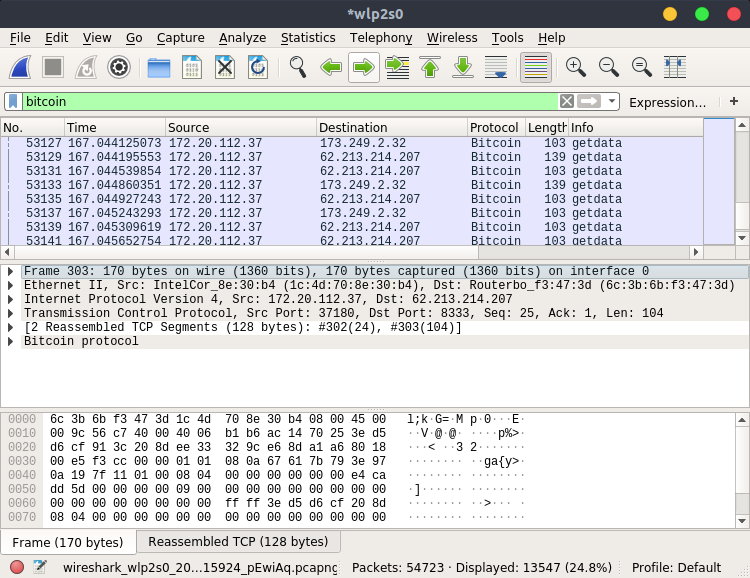
\includegraphics[width=15cm]{./resources/wireshark0.png}
\end{center}

\subsection{Estructura general}
Los nodos de Bitcoin se conectan entre ellos por TCP. Normalmente, los nodos buscan mensajes en el puerto 8333, aunque esto puede ser modificado. Cada mensaje de la red tiene una estructura definida.

\begin{table}[h]
\begin{tabular}{|C{2.8cm}|C{2.5cm}|L{7.5cm}|C{1.6cm}|}
\hline
\multicolumn{1}{|c}{\cellcolor[HTML]{81c784}\textbf{Descripción}} & \multicolumn{1}{|c}{\cellcolor[HTML]{81c784}\textbf{Tipo de dato}} & \multicolumn{1}{|c}{\cellcolor[HTML]{81c784}\textbf{Comentarios}} & \multicolumn{1}{|c|}{\cellcolor[HTML]{81c784}\textbf{Tamaño}} \\
\hline
magic & \texttt{uint32\_t} & Valor mágico indicando la red de origen del mensaje, y usado para buscar el estado del siguiente mensaje cuando el estado del stream no se conoce. & 4 bytes \\
\hline
command & \texttt{char[12]} & String ASCII identificando el contenido del paquete & 12 bytes \\
\hline
length & \texttt{uint32\_t} & Longitud del payload en número de bytes & 4 bytes \\
\hline
checksum & \texttt{unit32\_t} & Primeros 4 bytes de $sha256(sha256(payload))$ & 4 bytes \\
\hline
payload & \texttt{uchar[]} & La información que se quiere transmitir & \\
\hline
\end{tabular}
\end{table}
\pagebreak
El número mágico de 4 bytes para la red Bitcoin es \texttt{0xD9B4BEF9}, aquí lo vemos en \emph{little endian}:

\begin{center}
	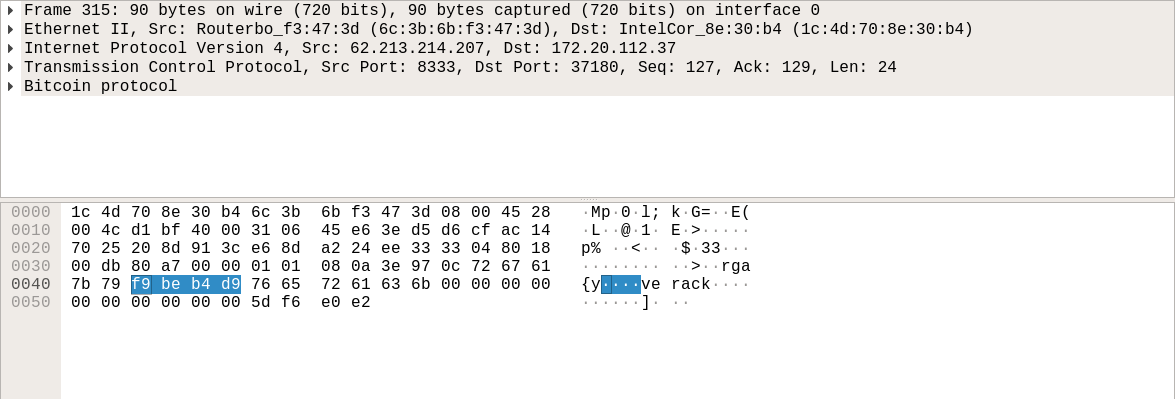
\includegraphics[width=16cm]{./resources/wireshark1.png}
\end{center}

Tras el número mágico, aparece un conjunto de 12 bytes, que describen el comando que es enviado en el mensaje, usualmente un texto ASCII. Por ejemplo, en la captura anterior vemos que se trata de un mensaje \texttt{verack}. En la documentación del protocolo Bitcoin podemos ver que se trata del mensaje enviado como respuesta a \texttt{version}.

\begin{center}
	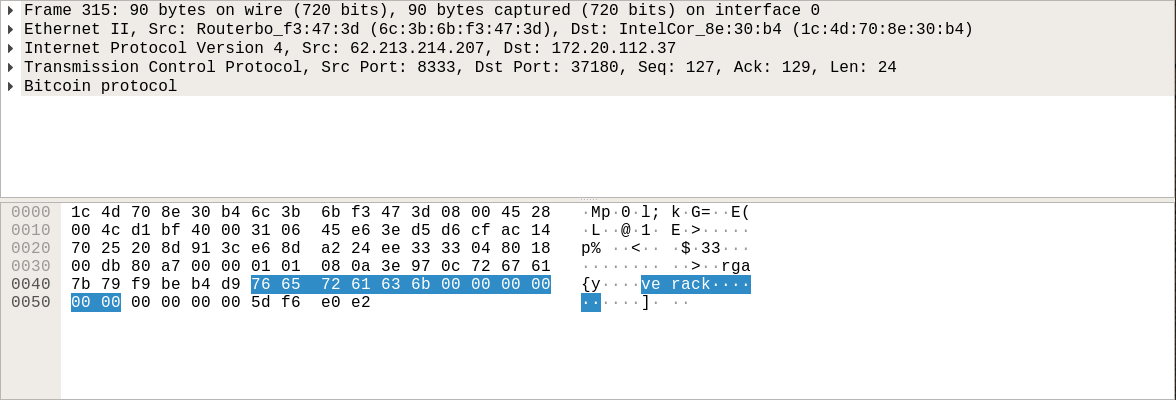
\includegraphics[width=16cm]{./resources/wireshark2.png}
\end{center}

\subsection{Analizando un mensaje: \texttt{block}}

Una vez que hemos visto la estructura general de un mensaje en Bitcoin, veamos con más detenimiento un mensaje, esta vez de tipo \texttt{block}.

Estos mensajes se generan como respuesta a un mensaje \texttt{getdata}, que requiere información de una transacción a partir del hash de un bloque.

Buscaremos un mensaje \texttt{block} en Wireshark, uno de ellos es el mensaje interceptado número 28681. Nótese en la captura siguiente que el mensaje anterior, el 28680, es un \texttt{getdata}.

Del mismo modo, podemos apreciar cómo todos los campos especificados anteriormente se encuentran en el mensaje (número mágico, comando, longitud, etc.).

\begin{center}
	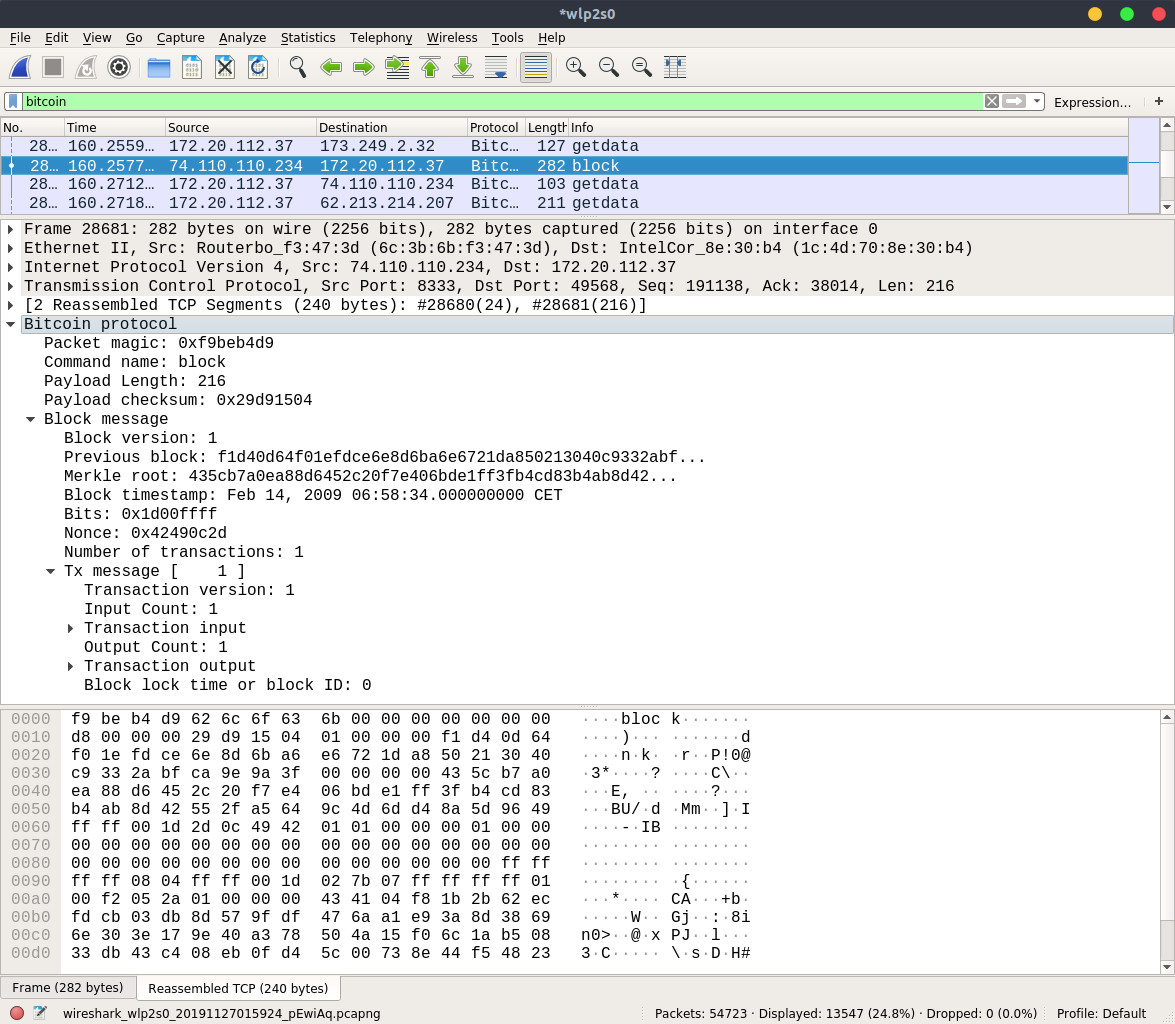
\includegraphics[width=16cm]{./resources/wireshark3.png}
\end{center}

Centrémonos, sin embargo, en el \emph{payload}, en la información que el mensaje pretende enviar. ¡Tenemos la cabecera del bloque que habíamos visto antes! Simplemente, añadimos dos campos más:

\begin{table}[h]
\begin{tabular}{|C{2.8cm}|C{2.5cm}|L{7.5cm}|C{1.6cm}|}
\hline
\multicolumn{1}{|c}{\cellcolor[HTML]{81c784}\textbf{Descripción}} & \multicolumn{1}{|c}{\cellcolor[HTML]{81c784}\textbf{Tipo de dato}} & \multicolumn{1}{|c}{\cellcolor[HTML]{81c784}\textbf{Comentarios}} & \multicolumn{1}{|c|}{\cellcolor[HTML]{81c784}\textbf{Tamaño}} \\
\hline
txn\_count & \texttt{var\_int} & Número de transacciones & 1+ bytes \\
\hline
txns & \texttt{tx[]} & Bloques de transacción, en el formato de un comando ``tx'' & \\
\hline
\end{tabular}
\end{table}
\pagebreak
Vemos que estos campos, en efecto, contienen información de transacciones, de acuerdo a la codificación explicada en la sección anterior:

\begin{center}
	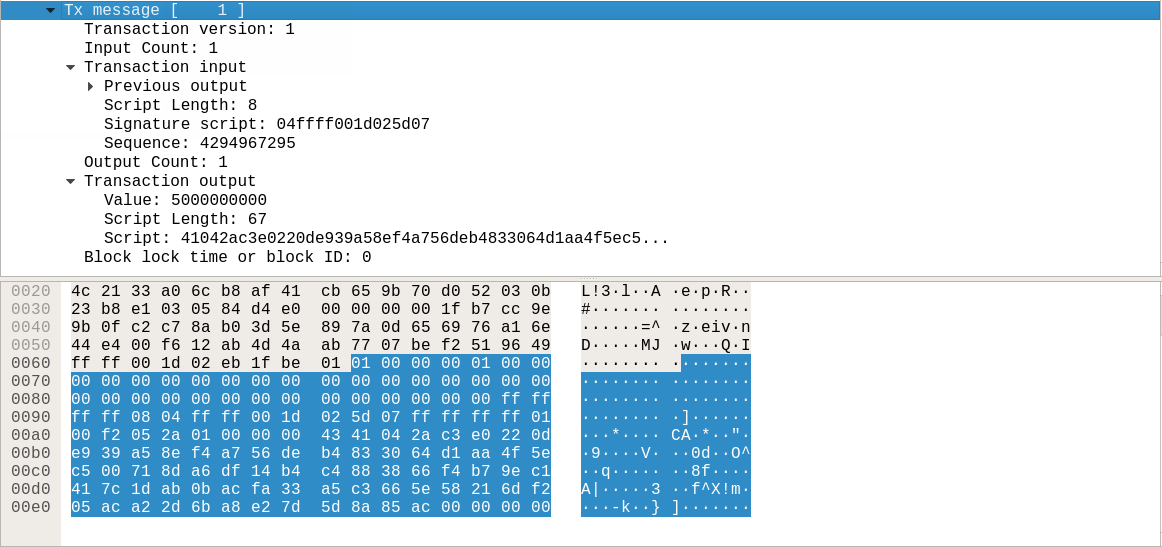
\includegraphics[width=16cm]{./resources/wireshark4.png}
\end{center}

Analizando el mensaje, vemos que la transacción era por valor de 5000000000 Satoshis, es decir, 50 BTC. Además, vemos que esta transacción no es resultado de un \emph{mining}, pues el input no es todo cero.

\pagebreak
\part{Bibliografía}

\begingroup
\renewcommand{\section}[5]{}%
%\renewcommand{\chapter}[2]{}% for other classes

\begin{thebibliography}{11}
	\bibitem{1}
	S. Nakamoto. \emph{Bitcoin: A Peer-to-Peer Electronic Cash System}.
	\\\url{https://bitcoin.org/bitcoin.pdf}
	\bibitem{2}
	D. Selmanovic. \emph{Bitcoin and cryptocurrency algorithms implementation tutorial}, Toptal Developers.
	\\\url{https://www.toptal.com/bitcoin/cryptocurrency-for-dummies-bitcoin-and-beyond}
	\bibitem{3}
	3Blue1Brown, \emph{But how does Bitcoin actually work?}.\\\url{https://www.youtube.com/watch?v=bBC-nXj3Ng4}
	\bibitem{4}
	Bitcoin Core.\\\url{https://bitcoincore.org/}
	\bibitem{5}
	Bitcoin Protocol Documentation.\\\url{https://en.bitcoin.it/wiki/Protocol_documentation}
	\bibitem{6}
	Binance Academy, \emph{Proof of Burn explicada}.
	\\\url{https://www.binance.vision/es/blockchain/proof-of-burn-explained}
	\bibitem{7}
	HackerNoon, \emph{Proof of Work, Proof of Burn and Proof of Stake}.\\\url{https://hackernoon.com/proof-of-work-proof-of-stake-and-proof-of-burn-6823eac2776e}
\end{thebibliography}
\endgroup

\vspace{9cm}
\begin{nota}
	Los enlaces que aparecen aquí fueron actualizados a fecha de 27 de noviembre de 2019. Es posible que sufran algún tipo de modificación, incluso llegando a no estar disponibles.
	
\end{nota}

\end{document}
